\documentclass[titlepage = firstcover]{scrartcl}
\usepackage[aux]{rerunfilecheck}
\usepackage{fontspec}
\usepackage[main=ngerman, english, french]{babel}

% mehr Pakete hier
\usepackage{expl3}
\usepackage{xparse}
\usepackage{float}

%Mathematik------------------------------------------------------
\usepackage{amsmath}   % unverzichtbare Mathe-Befehle
\usepackage{amssymb}   % viele Mathe-Symbole
\usepackage{mathtools} % Erweiterungen für amsmath
\usepackage[
  math-style=ISO,    % \
  bold-style=ISO,    % |
  sans-style=italic, % | ISO-Standard folgen
  nabla=upright,     % |
  partial=upright,   % /
]{unicode-math}% "Does exactly what it says on the tin."

% Laden von OTF-Mathefonts
% Ermöglich Unicode Eingabe von Zeichen: α statt \alpha

\setmathfont{Latin Modern Math}
%\setmathfont{Tex Gyre Pagella Math} % alternativ zu Latin Modern Math
\setmathfont{XITS Math}[range={scr, bfscr}]
\setmathfont{XITS Math}[range={cal, bfcal}, StylisticSet=1]

\AtBeginDocument{ % wird bei \begin{document}
  % werden sonst wieder von unicode-math überschrieben
  \RenewDocumentCommand \Re {} {\operatorname{Re}}
  \RenewDocumentCommand \Im {} {\operatorname{Im}}
}
\usepackage{mleftright}
\setlength{\delimitershortfall}{-1sp}

%Sprache----------------------------------------------------------
\usepackage{microtype}
\usepackage{xfrac}
\usepackage[autostyle]{csquotes}    % babel
\usepackage[unicode, pdfusetitle]{hyperref}
\usepackage{bookmark}
\usepackage[shortcuts]{extdash}
%Einstellungen hier, z.B. Fonts
\usepackage{booktabs} % Tabellen

%Defininierte funktionen
\DeclareMathOperator{\f}{xyz}

\ExplSyntaxOn % bequeme Syntax für Definition von Befehlen

\NewDocumentCommand \I {} {         %Befehl \I definieren,keine Argumente
  \symup{i}                         %Ergebnis von \I
} 
\NewDocumentCommand \dif { m m } % m = mandatory (Pflichtargument für \dif)
{
  \mathinner{\frac{\symup{d} #1}{\symup{d} #2}}
}

\ExplSyntaxOff % Syntax wieder ausschalten. Wichtig!


\begin{document}
\section{Begriffserklärung}
\begin{description}
\item{\textbf{Mittelwert}} \newline
    Der Mittelwert $\bar{x}$ ist der Wert der in der Mitte aller Daten liegt. Dabei geht es um die Werte der Daten und nicht um die Anzahl der Datenpunkte über und unter dem Wert. Um den Mittelwert zu bestimmen werden alle Datenwerte $x_n$ addiert und die Summe wird durch die Anzahl der Daten $N$ geteilt.
    \begin{equation}
        \langle x\rangle = \frac{1}{N} \sum \limits_{i=0}^{N}x_i
    \end{equation}
    Im Experiment kann es vorkommen dass der theoretisch berechnete Mittelwert nie genau gemessen wird.
\item{\textbf{Standardabweichung}} \newline
    Die Standardabweichung $\sigma$ gibt eine Abschätzung wie weit die Werte gestreut sind. Wenn alle Werte den gleichen Wert haben ist sie 0. Wenn die Werte weit gestreut sind ist die Standardabweichung groß.
    \begin{equation}
        \sigma = \sqrt{\sigma^2} = \sqrt{\langle x^2 \rangle -\langle x\rangle^2} = \sqrt{\frac{1}{N-1} \cdot \sum_{i=0}^{N} \left(x_i-\langle x \rangle\right)^2 }
    \end{equation}
\item{\textbf{Fehler und Standardabweichung}} \newline
    Der Fehler $\Delta x$ der Messwerte hängt zum Teil von der Streuung der Messwerte ab,er hängt aber auch von der Genauigkeit des Messinstruments ab. Die Standardabweichung liefert informationen wie die Werte gestreut sind, aber nicht wie genau die Einzelmessungen sind.
\end{description} 

\section{Volumenberechnung}
Für die Berechnung des Volumens eines Hohlzyliners gilt 
\begin{equation*}
    V = \pi (R_a^2 - R_i^2) \cdot h
\end{equation*}
Um den Fehler des Volumens zu berechnen gilt nach der Gauß'schen Fehlerfortpflanzung
\begin{align*}
    |\Delta V|&= \sqrt{ \left( \dif{V}{R_a} \Delta R_a \right)^2 + \left( \dif{V}{R_i} \Delta R_i \right)^2  + \left( \dif{V}{h} \Delta h \right)^2 } \\
              &= \sqrt{ \left( 2\pi h R_a  \right)^2 \Delta R_a^2 + \left( 2\pi h R_i \right)^2 \Delta R_i ^2 + \left( \pi (R_a^2 - R_i^2 )\right)^2 \Delta h^2 }
\end{align*}
Damit ergibt sich für das Volumen
\begin{equation*}
    V = \left(2500\pi \pm 25\sqrt{857}\pi\right) \; \text{cm}^3 ≈  \left(2500\pi \pm 732 \pi\right) \; \text{cm}^3 ≈  \left(785 \pm 230\right)\cdot 10^{1} \; \text{cm}^3
\end{equation*}
Und somit ein prozentualer Fehler von $\pm 29,3\%$

\newpage

\section{Lineare Regression}
\begin{table}[H]
    \centering
    \begin{tabular}{c c c}
        \toprule
        \textbf{Liniennummer} & Abstand $d$ & Spannung \\
        $N$\textsubscript{Linie} & m & V \\
        \midrule
        % 0.  6. 12. 18. 24. 30. 36. 42. 48
        % -19.5 -16.1 -12.4  -9.6  -6.2  -2.4   1.2   5.1   8.3
        1 & 0 & -19,5\\
        2 & 6 & -16,1\\
        3 & 12 & -12,4\\
        4 & 18 & -9,6\\
        5 & 24 & -6,2\\
        6 & 30 & -2,4\\
        7 & 36 & 1,2\\
        8 & 42 & 5,1\\
        9 & 48 & 8,3\\
        \bottomrule
    \end{tabular}
    \caption{Liniennummer, berechneter Abstand und Spannung}
    \label{tab:Wertetabelle}
\end{table}
Aus den Liniennummern \textbf{$N$\textsubscript{Linie}} wurden die Abstände \textbf{d} berechnet.\ref{eqn:abstand}
\begin{equation}
    d = (N\text{\textsubscript{Linie}}-1)\cdot 6 \text{mm}
    \label{eqn:abstand}
\end{equation}
Nun kann über eine Lineare Ausgleichsrechnung eine Funktion der Form $D(U) = m\cdot U + b$ an die Messwerte angenähert werden.
\begin{figure}[H]
    \center
    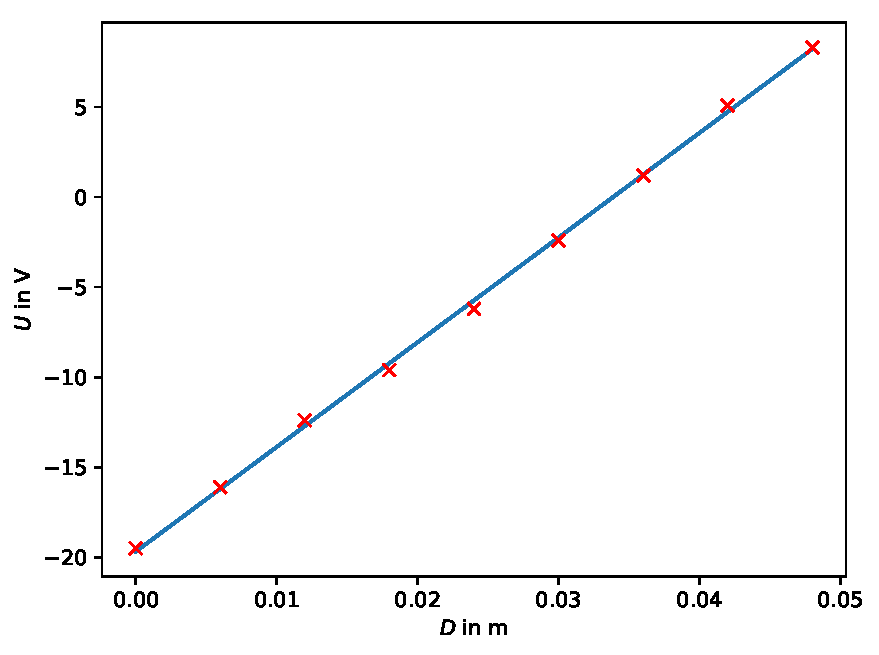
\includegraphics[width=0.6\textwidth]{build/plot.pdf}
    \caption{Plot}
    \label{tab:LF_D}
\end{figure}
Für die Parameter der Funkion ergibt sich damit
\begin{align*}
    m &= (0.001719 \pm 0.000020) \frac{\text{m}}{\text{V}}\\
    b &= \left(0.03386 \pm 0.00021\right) \text{m}
\end{align*}








\end{document}